\documentclass[conference,compsoc]{IEEEtran}
\usepackage[nocompress]{cite}
\usepackage[english]{babel}
\usepackage[utf8]{inputenc}
\usepackage{graphicx,wrapfig,lipsum}
\usepackage{xspace}
\usepackage{float}
\usepackage[breaklinks]{hyperref}
\usepackage{soul}
\usepackage{mathtools}
\usepackage{hyperref}
\usepackage{comment}
\DeclarePairedDelimiter\ceil{\lceil}{\rceil}
\DeclarePairedDelimiter\floor{\lfloor}{\rfloor}
\usepackage{array}
\newcolumntype{P}[1]{>{\centering\arraybackslash}p{#1}}

\graphicspath{ {img/} }

%Breaking urls by / and -
\def\UrlBreaks{\do\/\do-}

%rewriting the trademark commands to include and space after
\let\OldTexttrademark\texttrademark
\renewcommand{\texttrademark}{\OldTexttrademark\xspace}%
\let\OldTextregistered\textregistered
\renewcommand{\textregistered}{\OldTextregistered\xspace}%

\makeatletter
\renewcommand\paragraph{\@startsection{paragraph}{4}{\z@}%
	{-2.5ex\@plus -1ex \@minus -.25ex}%
	{1.25ex \@plus .25ex}%
	{\normalfont\normalsize\bfseries}}
\makeatother
\setcounter{secnumdepth}{4} % how many sectioning levels to assign numbers to
\setcounter{tocdepth}{4}    % how many sectioning levels to show in ToC


\begin{document}

\title{Meta volante \#1 - Buscando FLOPs entre las migajas}

\author{
	\IEEEauthorblockN{
		Vincent A. Arcila\IEEEauthorrefmark{1},
		Cristian Alzate\IEEEauthorrefmark{2},
		Alejandro Mc Ewen\IEEEauthorrefmark{3},
		Juan Nicolas Quintero\IEEEauthorrefmark{4}
	}
	\IEEEauthorblockA{
		\\
		Universidad EAFIT \IEEEauthorrefmark{1}\IEEEauthorrefmark{2}\IEEEauthorrefmark{3}\\
		Universidad del Rosario\IEEEauthorrefmark{4}\\
		Colombia\\
		\\
		\IEEEauthorrefmark{1}vaarcilal@eafit.edu.co,
		\IEEEauthorrefmark{2}calzateu@eafit.edu.co,
		\IEEEauthorrefmark{3}amce@eafit.edu.co,
		\IEEEauthorrefmark{4}juann.quintero@urosario.edu.co
	}
}

\IEEEtitleabstractindextext{
   \begin{abstract}
   		En el presente documento se describe el proceso de de implementación para la solución de la meta volante \#1. Este documento sirve como referencia para entender la experiencia del equipo 1 optimizando la ejecución de HPL.
   \end{abstract}
}

\maketitle
\IEEEdisplaynontitleabstractindextext

\section{Entorno del cluster}\label{OurOwnCluster}

\subsection{Hardware}\label{OurOwnCluster:HardwareEnvironment}
\begin{itemize}
	\item \textbf{Cantidad de nodos:} 2$\times$ProLiant SL230s Gen8.
	\item \textbf{Procesadores por nodo:} 2$\times$CPU Intel\textregistered Xeon\textregistered CPU. E5-2670, 8 núcleos por procesador, hyperthreading desactivado.
	\item \textbf{Controlador Infiniband: } Mellanox Technologies MT27500 Family ConnectX-3
	\item \textbf{Memoria por nodo:} 16 x 4GB DIMM DDR3 1333 M3T/s.
\end{itemize}

\subsection{Software}\label{OurOwnCluster:SoftwareEnvironment}

\begin{itemize}
    \item \textbf{Intel OneAPI} \cite{intel-oneapi}.
	\item \textbf{HPL 2.3 Intel version} \cite{intel-hplversion}.	
	\item \textbf{Operating system:} Centos 8.2 \cite{centos}.
	\item \textbf{BLAS:} BLAS en MKL \cite{intel-mkl-blas}.
	\item \textbf{MPI:} Intel MPI \cite{intel-mpi}.
\item \textbf{Compilador:} Intel C Compiler (envuelto por Intel MPI) \cite{intel-compiler}.
	\item \textbf{NFSv4} \cite{nfs-tutorial}.
	\item \textbf{Manejador de recursos}: Slurm 20.11.8 \cite{slurm20-11-8}.
	\item \textbf{Drivers de Infiniband}: Mellanox OFED 4.9 LTS.
\end{itemize}

\section{Estudio de performance}

El máximo performance teórico de nuestro cluster está determinado por la siguiente fórmula. 

\begin{equation} \label{eq:1}
	R_{peak} = \#nodos \times \frac{\#cpus}{nodo} \times \frac{\#nucleos}{cpu} \times \frac{ciclos}{segundo} \times \frac{FLOPs}{ciclo} 
\end{equation}

En nuestros nodos se tenia activado Turbo Boost para aumentar la frecuencia de los procesadores. Si bien en otros clusters se vio que la frecuencia podía mantenerse en 2.9GHz cuando se ejecuta HPL, en nuestros nodos el promedio de frecuencia por núcleo es 2.7GHz.

En nuestros nodos el mejor set de instrucciones para operaciones vectoriales es AVX \cite{intel-avx}. Con precisión doble, AVX puede hacer 8 operaciones de punto flotante por ciclo \cite{wikichip-flops}.

Para nuestro sistema, se tenia el siguiente $R_{peak}$:

\begin{equation} \label{rpeak_two_node}
	R_{peak} = 2 \times 2 \times 8 \times 2.7 \times 10^{9} \times 8 = 691.2\ {GFLOP}/s
\end{equation}

\section{El camino a ser los mejores}

\begin{enumerate}
	\item \textbf{Backups}. Diarios, para que no se pierda nada importante.
	\item \textbf{Montar NFS}.
	\item \textbf{Instalar drivers de Mellanox}.
	\item \textbf{Instalar SLURM}. Esto nos sirvió para coordinar nuestras ejecuciones cuando se trabajo individualmente.
	\item \textbf{Instalar Intel}. Se instalo Intel OneAPI \cite{intel-oneapi} Base y HPC toolkits, que traían consigo Intel MPI \cite{intel-mpi} e Intel MKL \cite{intel-mkl-blas}. 
	\item \textbf{Resultados base}. Se ejecuto HPL usando MKL e Intel MPI usando la versión base de HPL. Estos resultados nos sirvieron para saber nuestro punto de partida cuando se uso el HPL de Intel.
	\item \textbf{Optimización con Intel HPL}. Es la fase donde empezamos a ejecutar  autotuners en masa que nos pudieran mostrar los valores óptimos de la configuracion de HPL.
\end{enumerate}

\subsection{Backups}
Al momento de trabajar con un cluster que tiene bastante tiempo de funcionamiento es posible perder el trabajo realizado, ya que puede fallar definitivamente, estropenado la información del disco \cite{Meta-Volante-0}. Para evitar que se arruine el progreso obtenido es recomendable hacer Backups frecuentemente. Nosotros decidimos hacerlos todos los días. Por lo tanto, estas copias se harán en el servidor \verb|cronos.eafit.edu.co| reservadas para el usuario \verb|proxyjump|. \cite{Meta-Volante-0}.

Para el trabajo se hicieron las sincronizaciones con Rsync. Esta es una herramienta para realizar sincronización de archivos remotos y locales, usando un algoritmo que solo copia los archivos que cambiaron, optimizando el uso de recursos en la máquina. Además, para ejecutar este trabajo automáticamente se programó un archivo bash que fue corrido desde \textit{Crontab}, el cual permite hacer tareas con la frecuencia que se elija mediante ciertos comandos \cite{crontab}. 

\subsection{Montar NFS}
Un \textit{sistema de archivos de red (NFS por su siglas en inglés)} permite acceder a un sistema de archivos remotos a través de la red, facilitando la administración de recursos en servidores centralizados \cite{nfs-tutorial}. Este sistema es requerido por MPI para su correcto funcionamiento. NFS funciona bastante bien para un número reducido de nodos, pero hay mejores opciones como GlusterFS o Lustre \cite{Meta-Volante-0}. Nuestro servidor NFS estuvo montado en el \verb|compute-1-1| y el cliente en \verb|compute-1-2|.

\subsection{Infiniband}


Infiniband es una conexión para acelerar la comunicación entre nodos. En la instalación de Infiniband se usó el driver Mellanox. Se instaló la versión SRC, de modo que nos permitiera compilar todos los paquetes para nuestra versión se kernel específica. Se activó en tiempo de instalación RDMA, NFSoRDMA e IPoIB. Se activó también la instalación de todos los paquetes que vienen con los drivers.

\subsection{Intel}
 Se instaló Intel porque puede compilar aplicaciones para que funcionen mejor con el hardware y además trae una versión optimizada de HPL. Instalar Intel es fácil, solo se descarga y se corre el bash para construirlo. Más adelante se mostrarán los flags de compilación y variables de ambiente para mejorar la compilación y ejecución de HPL con Intel.\cite{intel-oneapi}

\subsection{Paquetes} 

Para instalar estas aplicaciones y otras se tuvieron que incluir múltiples paquetes. Los paquetes que se instalaron fueron usados para poder instalar los drivers y las aplicaciones. Además se instalaron varios paquetes para optimizar la comunicación de los nodos. Todos los paquetes instalados están en el documento Paquetes.txt.zip.
\subsection{Slurm}
Slurm es un sistema de control para supercomputadores. Permite controlar los procesos de manera que corran con todos los recursos que necesitan. Slurm hay que instalarlo en los dos nodos. La instalación de Slurm se debe hacer después de instalar NFS. Además de esto hay que instalar \verb|munge| para usar su servicio de autenticación. Para compilar Slurm se usó \verb|march-native|, que optimiza la ejecución de Slurm.

Se configuró Slurm desactivando el soporte para \verb|cgroup|, para estar seguros que no se restringían los recursos en las ejecuciones.

\subsection{Montar NTP}
NTP es un protocolo usado para sincronizar los relojes de las computadoras dentro de una red. Para ello se usará la aplicación Chrony, la cual se instaló usando el manejador de paquetes. De esta forma, se sincronizó \verb|compute-1-1| a la hora oficial de Bogotá usando el servidor \verb|3.co.pool.ntp.org|. Después, se usó \verb|compute-1-1| como servidor para \verb|compute-1-2|.

\section{La mera optimización ganadora}
En esta sección se expandió sobre las técnicas ganadoras. Se intentó ver a HPL desde todos los ángulos posibles, intentando aumentar FLOPs con todas las herramientas que se tuvo.

\subsection{Archivo de configuración}

\begin{itemize}
	\item \textbf{N}: Este es parámetro que más impacta el resultado. Define el tamaño de la matriz. El objetivo debe ser siempre elegir el valor más grande que quepa en RAM para maximizar la proporción de computación efectiva \cite{studentasc}, sin causar que el sistema haga swapping. Hay que tener en cuenta que el sistema operativo ocupa espacio en memoria, por lo que la matriz no debe ocupar el 100\% de la RAM. El porcentaje óptimo de memoria a ocupar está alrededor del 80\% \cite{studentasc}.
	Existe una fórmula para hallar el N que representa el tamaño de la memoria:
    \begin{equation*}
        \sqrt{(TotalMem \times (1024^3) \times Nodos) /8}
    \end{equation*}
    
    Donde \textit{TotalMem} es el tamaño de la memoria en GB y \textit{Nodos} es el número de nodos. También se pued multiplicar por el factor que representa el porcentaje de memoria que se quisiera usar, por ejemplo, para el 90\% se tiene:
    
    \begin{equation*}
        \sqrt{(TotalMem \times (1024^3) \times Nodos) /8} \times 0.90
    \end{equation*}
    
    En nuestros nodos, había alrededor de 61.3 GiB libres en cada uno. No se puede utilizar completamente esta cifra, pues los buffers de memoria y MPI necesitan espacio. El N que usamos fue 125440, que ocupa $~117.2 GiB$ en total.
	
	\item \textbf{NB}: Define el tamaño del bloque para la distribución de datos. En general son menores a 256 y los mejores valores suelen ser múltiplos de 32 \cite{netlib-hpl-faq}. Además, se consideró que lo mejor es que N fuera divisible entre NB, para hacer un uso más eficiente de la memoria. Para este trabajo se estableció un valor de 256, ya que en varias fuentes se evidenció que era el mejor para nuestro procesador.
	
	\item \textbf{P$\times$Q}: El producto de \textbf{P} y \textbf{Q} es la cantidad de procesos que HPL va a utilizar. \textbf{Q} debe ser un poco mayor de \textbf{P}.
	
	Para la versión de Intel HPL, la cantidad óptima de procesos es la cantidad de sockets que se tienen. En nuestra configuración, el óptimo es 4.
	
	\item Panel Factorization: Hay tres opciones para factorizar el panel: left, crout, y right. Depende de la máquina de cual opción es la mejor. Para nuestros nodos la opción mas rápida fue right. Esto se puede modificar cambiando los PFACs.
    \item Recursion Factorization: Hay tres opciones para factorizar la recursión: left, crout, y right. Depende de la maquina cual es la mejor opción. Para nuestros nodos la opción más rápida fue right. Esto se puede modificar cambiando los RFACs.
    \item Panel Broadcast: Las mejores configuraciones de panel broadcast son increasing ring modified 1 y 2. Esto es porque mandan la información mucho más rápido al segundo nodo haciendo que toda la comunicación se mueva mas rápido.
    \item Look ahead: Este parámetro hace que el programa mande información al siguiente panel. Esto lo cambias modificando el parametro de depth. Puede mejorar la velocidad de procesamiento pero hay que tener cuidado porque toma mucha memoria.
    \item Update: Hay dos formas de update binary-exchange y long. Long normalmente es mejor para problemas mas grandes. Esto lo puedes cambiar cambiando el número del SWAP. Además se puso el threshold swapping en 128.
	
\end{itemize}

\subsection{Mantenimiento a la disipación de calor}
Durante algunas ejecuciones del HPL se obtuvieron diferentes advertencias por el recalentamiento de las CPUs. Para ello se hicieron algunas modificaciones en el BIOS del sistema, específicamente en una opción llamada \textit{Thermal configuration}, en la que se cambió el valor de \textit{Optimal cooling} a \textit{Maximum cooling}. Esto ayudó a que el sistema de refrigeración trabajara al máximo.

Sin embargo, analizando el comportamiento de la CPU se pudo envidenciar que uno de los procesadores de uno de los servidores tenía menor frecuencia que el otro procesador, y la diferencia de FLOPS era lo suficientemente relevante como para hacer algo al respecto. Hay que tener en cuenta que la frecuencia está directamente relacionada con el performance.

Por tal motivo, se pensó que el calor podría estar influyendo en el comportamiento del procesador, entonces se revisó la temperatura de cada uno con iLO. Allí se pudo comprobar que el procesador con menor rendimiento tenía una temperatura más elevada que el otro.\\

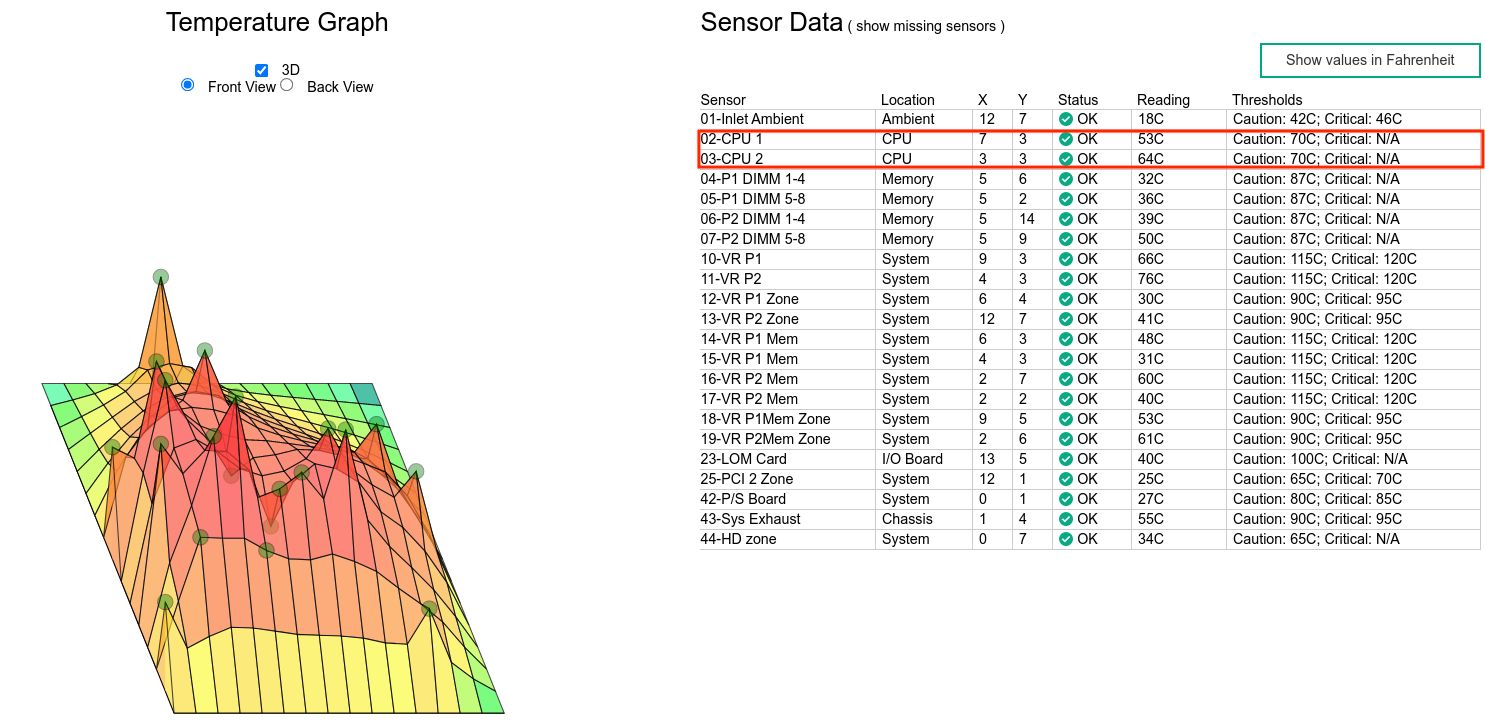
\includegraphics[width=8cm]{Temperatura.png}

Para tratar este problema lo mejor que se pensó fue cambiar la pasta de disipación de calor en cada una de los procesadores, entonces se realizó mantenimiento a estos en el centro de computación científica Apolo de la universidad EAFIT.\\


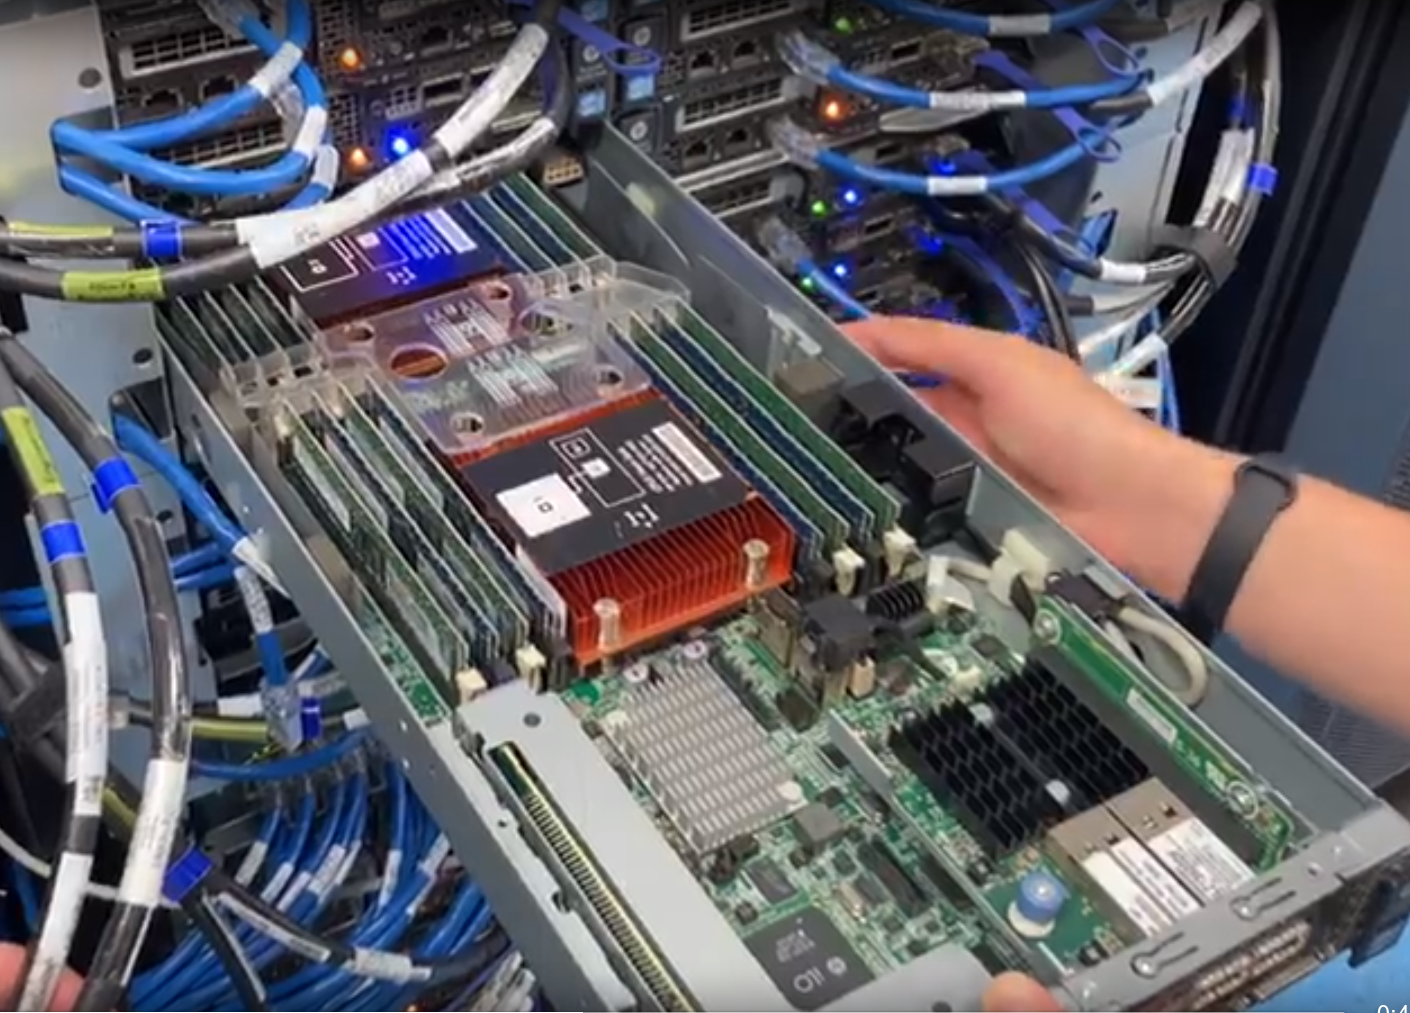
\includegraphics[width=8cm]{Compute-1-1.png}

\subsection{Flags de compilación}
Para optimizar la compilación de HPL de Intel se usaron varias flags de compilación.

\begin{itemize}
    \item -Ofast: Es una flag que incluye varias otras flags que son -O3, -no-prec-div, y -fp-model fast=2. -O3 optimiza el programa para algoritmos que tienen complejidad $ O(n^3)$. -no-prec-div le quita precisión a las operaciones de punto flotante. -fp-model fast=2 hace que el programa corra lo mas rápido posible.
    \item -xHost: Le dice al compilador que produzca instrucciones para el host.\cite{intel-xhost}
    \item -ansi-alias: Pone las reglas de ANSI en effecto.
    \item -fdefer-pop: Quita las funciones justo cuando retornan sus valores.
    \item -foptimize-sibling-calls: Optimiza las funciones de recursión de cola.
    \item -mbranches-within-32B-boundaries: Fusiona las ramas con limites 32-byte para mejorar rendimiento.
    \item -ip: Determina si están habilitadas las optimizaciones entre procedimientos adicionales para la compilación de un solo archivo.
    \item -qoverride-limits: Deja sobreponer sobre unos limites del compilador. Previene uso excesivo de la memoria.
    \item -use-intel-optimized-headers: Determina si el directorio de encabezados de rendimiento se agrega a la lista de búsqueda de ruta.
    \item -pcn 64: Pone la precisión de los número flotante en doble.
    \item -mkl=parallel: Importa la librería de paralelo del Math Kernel Library.
    \item -Wall: Pone diagnósticos de warning y error.
    \item -fPIC: Determina si el compilador código es de posición independiente.
\end{itemize}

\subsection{Swappinness a 0}
El swappinness es la tendencia del kernel de Linux a mover los datos de la memoria principal a la memoria SWAP. El kernel tiene un parámetro que determina el swappinnes. Se configuró para que no hiciera swapping a menos que fuera estrictamente necesario. Esto es útil porque en los casos en que HPL hace que la RAM quede con 1\% de memoria, que asegura de que no se estarán moviendo datos de HPL a SWAP, lo que dañaría dramáticamente el performance.

\subsection{Binding y Pinning}
 Una de las arquitecturas más comunes que se pueden encontrar hoy en día para las memorias es Non-Uniform Memory Access (NUMA). En esta cada nodo NUMA tiene su grupo de memorias RAM. La velocidad de acceso a memoria no solamente esta ligado a la jerarquía de memoria, sino también al lugar donde se encuentre el dato que se quiera acceder \cite{Meta-Volante-0} Por lo tanto, las aplicaciones de HPC pueden ser optimizadas mediante una técnica llamada \textit{binding} o \textit{pinning} fijando cómo se distribuyen los subprocesos en la memoria. Estos son fijados (pinned) con ciertas variables de entorno en MPI. En nuestro caso se utilizan dos \textit{I\_MPI\_PIN\_DOMAIN} que define un conjunto separado de CPUs en un solo nodo (dominio) y \textit{I\_MPI\_PIN\_ORDER} que indica el orden en el que los procesos MPI se asociarán con los dominios \cite{biding-pinning}. Dichas variables se inicializaron con los siguientes comandos:

 \begin{itemize}
 \item export I\_MPI\_PIN\_DOMAIN="numa"
 \item export I\_MPI\_PIN\_ORDER="compact"
 \end{itemize}

La opción "numa" indica que los procesos se mantienen dentro de un dominio NUMA. Mientras que "compact" asigna los hilos de forma que queden lo más cercanos posible.

\subsection{Variables de ambiente de MPI}

Se utilizó el protocolo de datagramas de usuario (UDP) para realizar el intercambio de mensajes de MPI debido a que es una alternativa mas escalable que consume menos memoria, este se activó utilizando los comand:\cite{hpl_params_intel}
\begin{itemize}
    \item export I\_MPI\_FABRICS=shm:dapl
    \item export I\_MPI\_DAPL\_UD=1
\end{itemize}
Para que se haga la transferencia utilizando RDMA se utilizó el comando:
\begin{itemize}
    \item export I\_MPI\_DAPL\_UD\_PROVIDER=ofa-v2-ib0
\end{itemize}
Se deshabilitó la opción de utilizar una fábrica de comunicación distinta de DAPL en caso de no poder inicializarla mediante el comando:
\begin{itemize}
    \item export I\_MPI\_FALLBACK=0
\end{itemize}
Se quería ver la cantidad de datos enviada por cada proceso, así como información de tiempos en las funciones de MPI, esto se realizo usando:
\begin{itemize}
    \item export I\_MPI\_STATS=1-20
\end{itemize}
Para guardar esa información se eligió una carpeta usando
\begin{itemize}
    \item export I\_MPI\_STATS\_FILE=$<$path de la carpeta$>$
\end{itemize}
Se estableció el número de procesos por nodo en 4 utilizando:
\begin{itemize}
    \item export I\_MPI\_PERHOST=4
\end{itemize}
Para evitar que el agendador de MPI establezca el número de procesos por nodo físico y que sea el que se estableció se debe deshabilitar el asignador de procesos usando:
\begin{itemize}
    \item export I\_MPI\_JOB\_RESPECT\_PROCESS\_\\PLACEMENT=0
\end{itemize}
También se realizaron optimizaciones sobre los algoritmos utilizados para realizar ciertas operaciones de MPI que se utilizan en HPL. Estas fueron:
\begin{itemize}
    \item \textbf{Allgather y allgatherv:}\\
    Para realizar esta operación el algoritmo ring resulta ser mas eficiente para mensajes de más de 512K y cuando se transmiten mensajes de menor longitud el algoritmo recursive doubling es mejor. Para establecer estos algoritmos se utilizan los comandos:\\
    \begin{itemize}
        \item export I\_MPI\_ADJUST\_ALLGATHER=”1:0-524288;3”
        \item export I\_MPI\_ADJUST\_ALLGATHERV=”1: 0-524288;3”
    \end{itemize}
    \item \textbf{Reduce:}\\
    Para operaciones con datos de menos de 2Kb el algoritmo binomial resulta más eficiente mientras que para operaciones con mas tamaño de datos es más eficiente el algoritmo de Rabenseifner, esto se estableció con el comando:
    \begin{itemize}
        \item export I\_MPI\_ADJUST\_REDUCE=”2:0-2048;5”
    \end{itemize}
    \item \textbf{Allreduce:}\\
    El caso de la operación allreduce es similar al de reduce, sin embargo el algoritmo más eficiente con menos de 2Kb es el algoritmo recursive doubling, se estableció con:
    \begin{itemize}
        \item export I\_MPI\_ADJUST\_ALLREDUCE=”1:0-2048;2”
    \end{itemize}
    \item \textbf{Broadcast:}\\
    En el caso del broadcast el algoritmo que nos da un mejor performance con mensajes de menos de 12 Kb resulta ser el binomial, se estableció con:
    \begin{itemize}
        \item export I\_MPI\_ADJUST\_BCAST=”1:1-12288”
    \end{itemize}
\end{itemize}

Finalmente se hizo que la ejecución corriera sobre los 2 nodos que fueron asignados utilizando slurm mediante los comandos:
\begin{itemize}
    \item export I\_MPI\_HYDRA\_HOSTS\_GROUP=compute-1-[1-2]
    \item export I\_MPI\_HYDRA\_BOOTSTRAP=slurm
\end{itemize}

\subsection{BIOS}

La configuración que se realizó en el BIOS fue la siguiente:

\begin{itemize}
    \item \textbf{Turbo Boost:} Enabled
    \item \textbf{Hp power profile:} Maximum performance
    \item \textbf{HP power regulator:} High performance 
    \item \textbf{Thermal Shutdown:} Disabled
    \item \textbf{Thermal configuration:} Maximum cooling
    \item \textbf{HP power profile:} Maximum performance
    \item \textbf{Thermal configuration:} Maximum cooling
    \item \textbf{ACPI SLIT preferences}
    \item \textbf{Intel performance counter monitor:} Enabled
    \item \textbf{Thermal Shutdown:} Disabled
\end{itemize}//
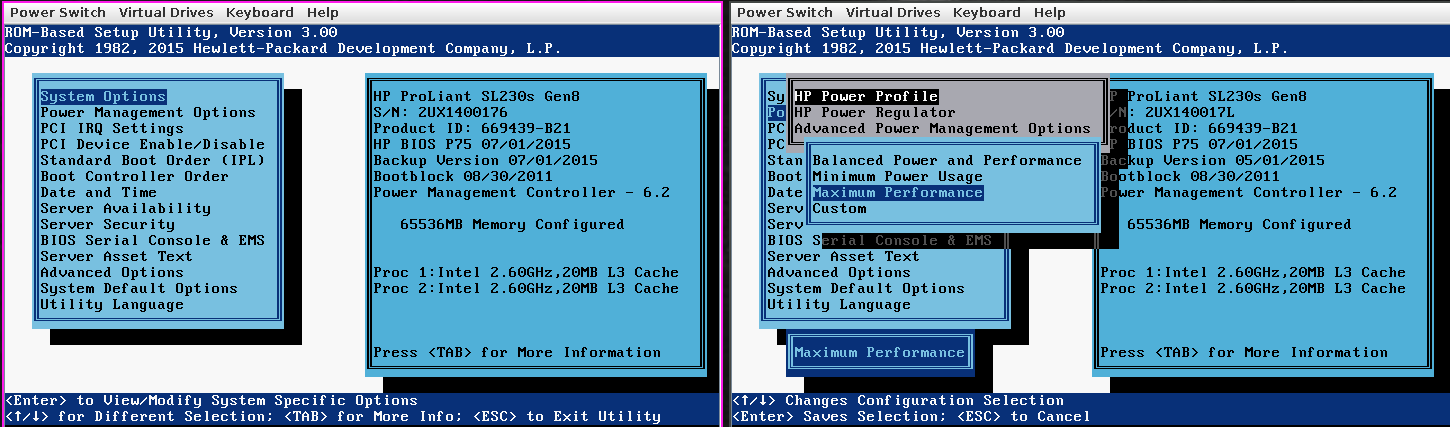
\includegraphics[width=8cm]{BIOS.png}

Los cambios realizados respecto a la configuración predeterminada fueron activar el maximun cooling, habilitar las ACPI SLIT preferences, el Intel performance counter monitor y deshabilitar el thermal shutdown.

\subsubsection{Mejoras con BIOS}

Al realizar los cambios en el BIOS en uno de los nodos (compute 1-2), se pudo observar una mejora en la velocidad de los ciclos con respecto al otro nodo (compute 1-1).

\subsection{Infiniband y modo datagrama}

El modo datagram es una configuración que tienen las tarjetas infiniband para modificar la manera en la que maneja los paquetes IP. El equipo 3 y notros usamos tests de ancho de banda de Infiniband juntos, para determinar cuál de las 2 opciones es mejor; el modo datagram o el modo connected. 

Haciendo tests con qperf \cite{tutorial-qperf}, se determino que el modo datagrama arroja un mayor ancho de banda.

\subsection{Eliminar servicios que sobran}

Se eliminaron servicios de RPC utilizando el comando:
\begin{itemize}
    \item systemctl mask --now rpc-statd.service rpcbind.service rpcbind.socket
\end{itemize}
También se eliminaron los siguientes servicios y daemons:
\begin{itemize}
    \item \textbf{polkit:} Servicio para manejar la autenticación en el SO.
    \item \textbf{crond:} Daemon que ejecuta periodicamente scripts en el SO.
    \item \textbf{chronyd:} Servicio de sincronización del reloj.
    \item \textbf{gssproxy:} Daemon para manejar acceso a credenciales GSSAPI.
    \item \textbf{rsyslog:} Servicio para recolectar logs de otros servicios.
    \item \textbf{sssd:} Daemon de servicios de sistema de seguridad.
    \item \textbf{munge:} Servicio que se encarga de la autenticación de slurm.
    \item \textbf{slurmd:} Servicio de monitoreo de tareas corriendo en un nodo.
    \item \textbf{slurmctld:} Servicio que monitorea otros daemons de slurm.
\end{itemize}
Estos se eliminaron con el comando:
\begin{itemize}
    \item systemctl stop polkit crond chronyd gssproxy rsyslog sssd munge slurmd slurmctld
\end{itemize}

\section{Resultado sorprendente}

Después de todo este trabajo de optimización se pudo obtener un resultado 642.747 GFLOPs, equivalente a una eficiencia de 92.99\%.\\

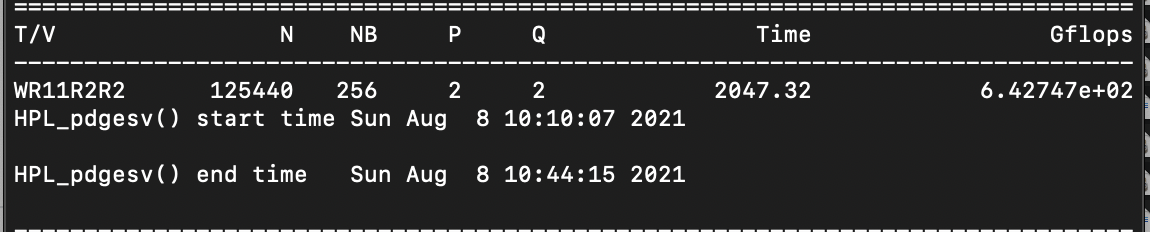
\includegraphics[width=8cm]{GFLOPS642.png}

\bibliographystyle{IEEEtran}
\bibliography{bibliography}

\end{document}
